% Chapter 1

\chapter{Introduction} % Main chapter title

\label{Chapter1} % For referencing the chapter elsewhere, use \ref{Chapter1} 

%----------------------------------------------------------------------------------------

% Define some commands to keep the formatting separated from the content 
\newcommand{\keyword}[1]{\textbf{#1}}
\newcommand{\tabhead}[1]{\textbf{#1}}
\newcommand{\code}[1]{\texttt{#1}}
\newcommand{\file}[1]{\texttt{\bfseries#1}}
\newcommand{\option}[1]{\texttt{\itshape#1}}
\setcounter{secnumdepth}{4}
%----------------------------------------------------------------------------------------

\section{Thesis Statement. Background and motivation}

\setlength{\parindent}{0.5cm} During the last decade, the use of phase change materials has been growing in the automotive industry. 

\noindent These substances release or absorb large amounts of latent heat when they go through a change in their physical state, as the material reaches its specific phase change temperature. Thus, in the process of latent heat release or absorption, the temperature of the phase change material (PCM) remains constant. Therefore, PCMs are considered to be efficient in terms of thermal storage. 

\noindent However, some of these PCM's may present physical effects which most of the times require special conditions for the containers in where they are placed. Thus, in such geometries, problems involving, i.e., solidification are of considerable relevance. And this is mainly due to a volumetric expansion originated by the thermal effects within the PCM which at its turn, generates stresses in the tank in which is bottled up.

\noindent On that basis, this master's thesis main objective aims to study different numerical techniques to represent solidification process and, specially, pure water phase change. This is accomplished by first stuying the physics of a pure convective solver. That will bring a new solver with a rather different gravity-related term and a polynomial density variation purely temperature dependent. This is validated against literature.
\begin{figure}[h!]
	\centering
	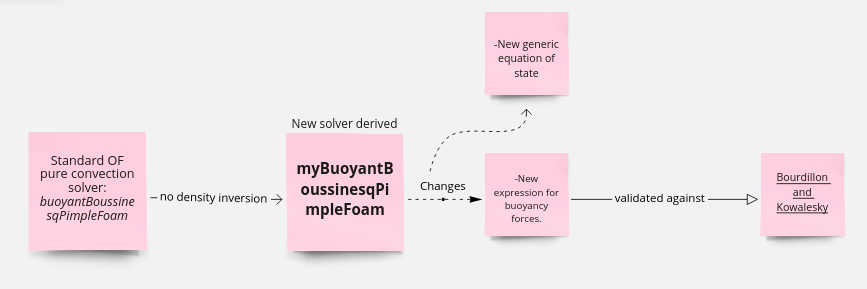
\includegraphics[width=1\linewidth]{buoyancy_roadmap.png}
	\caption{Workpath for buoyancy effects study.} 
	\label{1.1fig}
\end{figure}
\clearpage
\noindent And later, imlementing an enthalpy-porosity technique within the frame of a multi-phase incompressible solver based on volume-of-fluid (VOF) method for interface tracking. The objective of this first stage is to apply the latent heat as source term in the energy equation. 
\begin{figure}[h!]
	\centering
	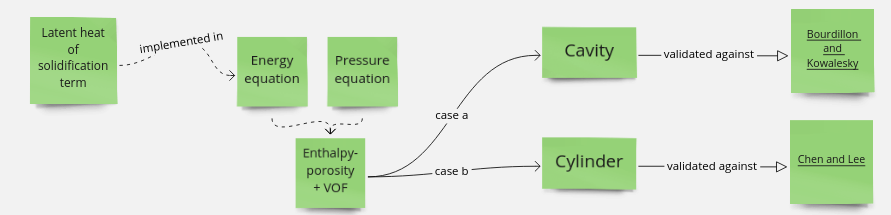
\includegraphics[width=1\linewidth]{EP_roadmap.png}
	\caption{Workpath for latent heat implementation in enthalpy-porosity model.} 
	\label{1.2fig}
\end{figure}
\newline
On a second stage of the thesis, a 2D semi-empirical model based on the work of Lee is adapted to account for the nucleation characteristics occured during the water phase transition. This is implemented within the same solver based on the technique of VOF as in the previous case.
\begin{figure}[h!]
	\centering
	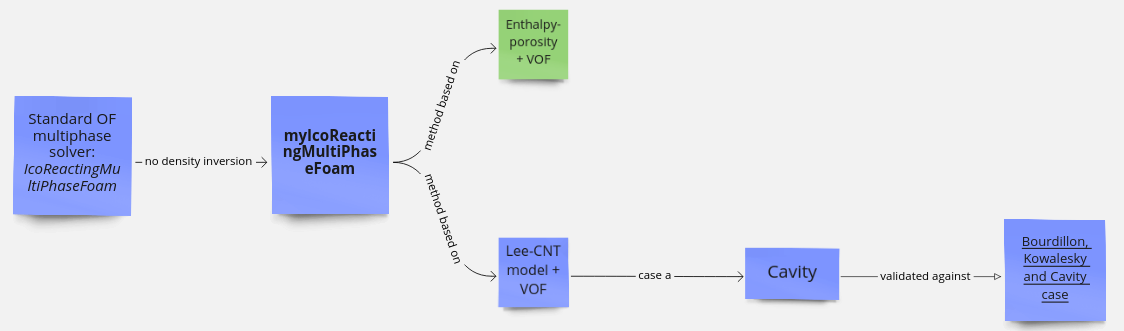
\includegraphics[width=1\linewidth]{icoreacting_roadmap.png}
	\caption{Workpath for nucleation theory implementation in Lee model.} 
	\label{1.3fig}
\end{figure}
\newline
\noindent The final stage of this thesis is devoted to an implementation of a multiregion solver to calculate conjugate heat transfer problems between solid and fluid zones with the singularity of being, the fluid zone, capable of handling phase change materials. Both models are validated against literature.
\clearpage
\begin{figure}[h!]
	\centering
	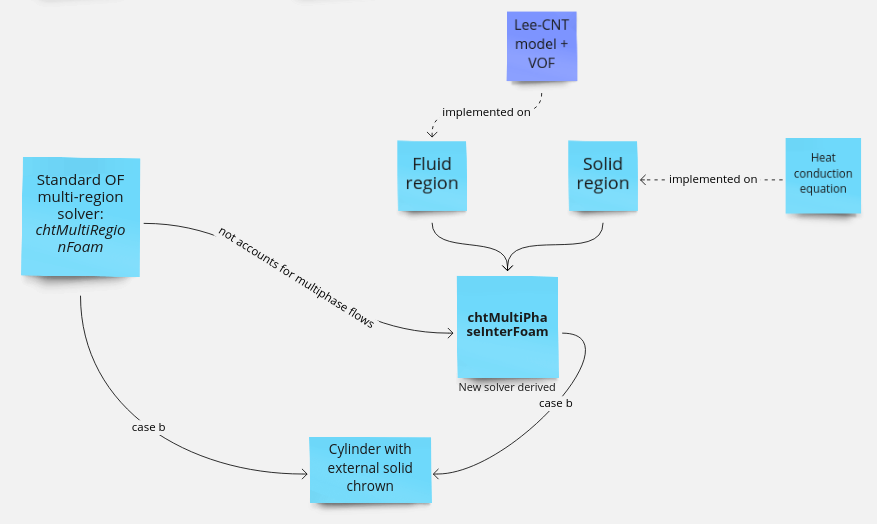
\includegraphics[width=1\linewidth]{cht_roadmap.png}
	\caption{Workpath for conjugate heat transfer implementation.} 
	\label{1.4fig}
\end{figure}

\noindent The next chapters are mainly focused on describing phase change phenomena and heat transfer mechanisms used along the completion of this master's thesis.


%----------------------------------------------------------------------------------------
\clearpage
\section{Phase Change Process}
\setlength{\parindent}{0.5cm} The phase change is usually modelled by a sudden change in enthalpy per unit of temperature generated within a narrow temperature range near the freezing point. Often, this process is assumed to behave in a characteristic temperature, as shown in Fig. \ref{1.5figa}, leading to a moving boundary problem. However, at a given critical temperature, both fluid and solid phases may coexist giving a state called mushy region as in Fig. \ref{1.5figb}. In this case, one speaks of a non-linear diffusion problem rather than a moving boundary problem \cite{krabbenhoft_damkilde_nazem_2006}. 
 
\begin{figure}[h!]
	\begin{subfigure}{0.50\textwidth}
		\centering
		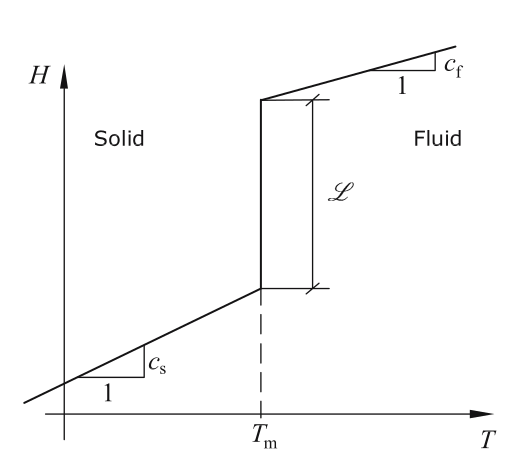
\includegraphics[width=1\linewidth]{isothermal_phasechange.png}\hfill
		\caption{Isothermal phase change.} 
		\label{1.5figa}
	\end{subfigure}
	\hfill
	\begin{subfigure}{0.50\textwidth}
		\centering
		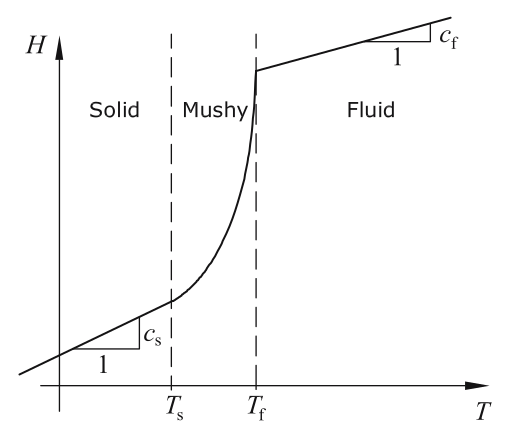
\includegraphics[width=1\linewidth]{non_iso_phasechange.png}	
		\caption{Non-isothermal phase change.}
		\label{1.5figb}
	\end{subfigure}
\caption{Phase change comparison.}
\label{1.5fig}
\end{figure}

\noindent As briefly introduced, two types of phase change are used to describe the way the latent heat is released or absorbed during freezing or melting processes:
\begin{itemize}
	\item \textbf{Non-isothermal phase change:} the phase change takes place within a temperature range yielding a transition zone between a solid and a liquid phase called mushy zone. Typically, the thickness of this region is straightfully proportional to the temperature range in wich the phase change occurs.
	\item \textbf{Isothermal phase change:} the phase change is arisen instantaneously at the melting temperature. The release or absorption of the latent heat occurs at this point in which, consequently, there is no transition zone between solid and liquid phases. At this point, there is a narrow line, mainly derived from the discretization of the computational domain, characterizing the phase change phenomena.
\end{itemize}

\noindent As an important remark, when the mushy region is sufficiently narrow, the isothermal assumption is usually a good approximation. However, despite of the fact of being a convenient approach it may lead to significant complication when it comes to numerical solution techniques. 
\newline
\noindent Along the next chapters, a more detailed description on existing techniques that deal with such non-trivial phenomena will be given.

\subsection{Water phase change}
\setlength{\parindent}{0.5cm} In a similar manner, the water phase change takes place. A complex interaction of the molecular forces generate water to behave in a curious way when it gets frozen into ice. The vast majority of substances, when they are cooled down, become more dense in the frozen state than when liquid. However, when cooled under a specific temperature, water begins to expand and, once it starts freezing, it becomes less dense than water. 

\subsection{Phase diagram of ice}
\setlength{\parindent}{0.5cm} When water begins to become ice, these ice crystals might undergo different kinds of structures. Called ice Ih, in the form of hexagonal ice and, manifested in six cornered snow flakes, is the natural ice generally found in earth. However, at lower pressures below 2 kbar, many other ice structures may exist.

\noindent The ice phase diagram shown in Fig. \ref{1.6fig}, points out the conditions of stability for all ice phases. As it is cleared out, the line between the water and ice Ih is an equilibrium line with a negative slope, consequence of having, the solid, lower density than the liquid. These equilibrium lines extend in the form of metastable phase boundaries into the area of stability of other ice phases.
Although there are at least 11 crystalline ice shapes, the only which is found in naturally on earth is the hexagonal form. 
\begin{figure}[h!]
	\centering
	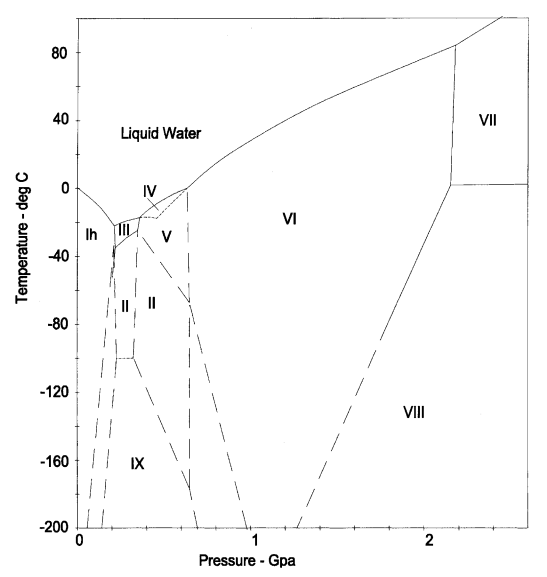
\includegraphics[width=0.5\linewidth]{phase_diagram_ice.png}
	\caption{Phase diagram of ice.} 
	\label{1.6fig}
\end{figure}
\newline
\noindent As a remark, the implication that there is a rise on the pressure would not propitiate ice formation at 0ºC, instead water would need to be cooled down.
\subsection{Properties of ice}
\setlength{\parindent}{0.5cm} Ice, when subjected to visible light conditions, is transparent and has the lowest index of refraction for the sodium spectrum of any known crystalline material, as pointed out by Akyurt et al. \cite{akyurt_zaki_habeebullah_2002}.

\noindent Mechanically, ice behaves like a viscoelastic material with a non linear law. Pollycrystalline ice subjected to stress, deforms elastically, followed by a transient creep and finally, a secondary creep in the form of steady viscous flow is obtained.

\noindent As described in \cite{akyurt_zaki_habeebullah_2002}, the surface of ice Ih near the melting point has many dangling broken bounds that boost the presence of a liquid-like layer and as a consequence, low friction on such surface. Variation of density of ice with phase at 110 K is described in the table shown below.

\begin{table}[h!]
	\begin{tabular}{@{}lllll@{}}
		\toprule[1pt]
		\textbf{Phase of ice} & \textbf{Density ($Mg/cm^{3}$)} \\ \midrule[2pt]
		\textbf{Ih} &  0.93 \\
		\textbf{II} &  1.18 \\
		\textbf{III} & 1.15  \\
		\textbf{IV} & 1.27  \\
		\textbf{V} &  1.24 \\
		\textbf{VI} & 1.33  \\
		\textbf{VII} & 1.56	\\
		\textbf{VII} & 1.56	\\
		\textbf{IX} & 1.16  \\
		\textbf{X} &  2.51 \\  \bottomrule[1pt]		
	\end{tabular}
	\centering
	\caption{Variation of ice density for every phase at 110K.}	
	\label{1.1tab}
\end{table}
\subsection{Freezing phenomena}
\setlength{\parindent}{0.5cm} Time-temperature diagram for freezing of pure water (ABCDE) and aqueous solutions (AB'C'D'E'), Fig.  \ref{1.7fig}, shows the physical process that occurs during the solidification. The first stage, from A to B, belongs to undercooling, also called supercooling, and it is arisen below the freezing point $T_f$, which is equal to the melting point, $T_m$. This point is referred to a non equilibrium point and it is analogous to an activation energy necessary for the nucleation process. Before nucleation process starts, pure water may need to be cooled down several degrees. At point B, the system nucleates and releases its latent heat faster than the heat which is being removed from itself.

\noindent From C to D, the horizontal axis shows the evolution of the crystal growth in time. At C, there exists the nucleation point and, from there through D, latent heat gets removed out of the system at constant temperature. In this way, the mixture, which is in a partially frozen state, does not cool until all the potentially freezable water has crystallized.
\clearpage

\begin{figure}[h]
	\centering
	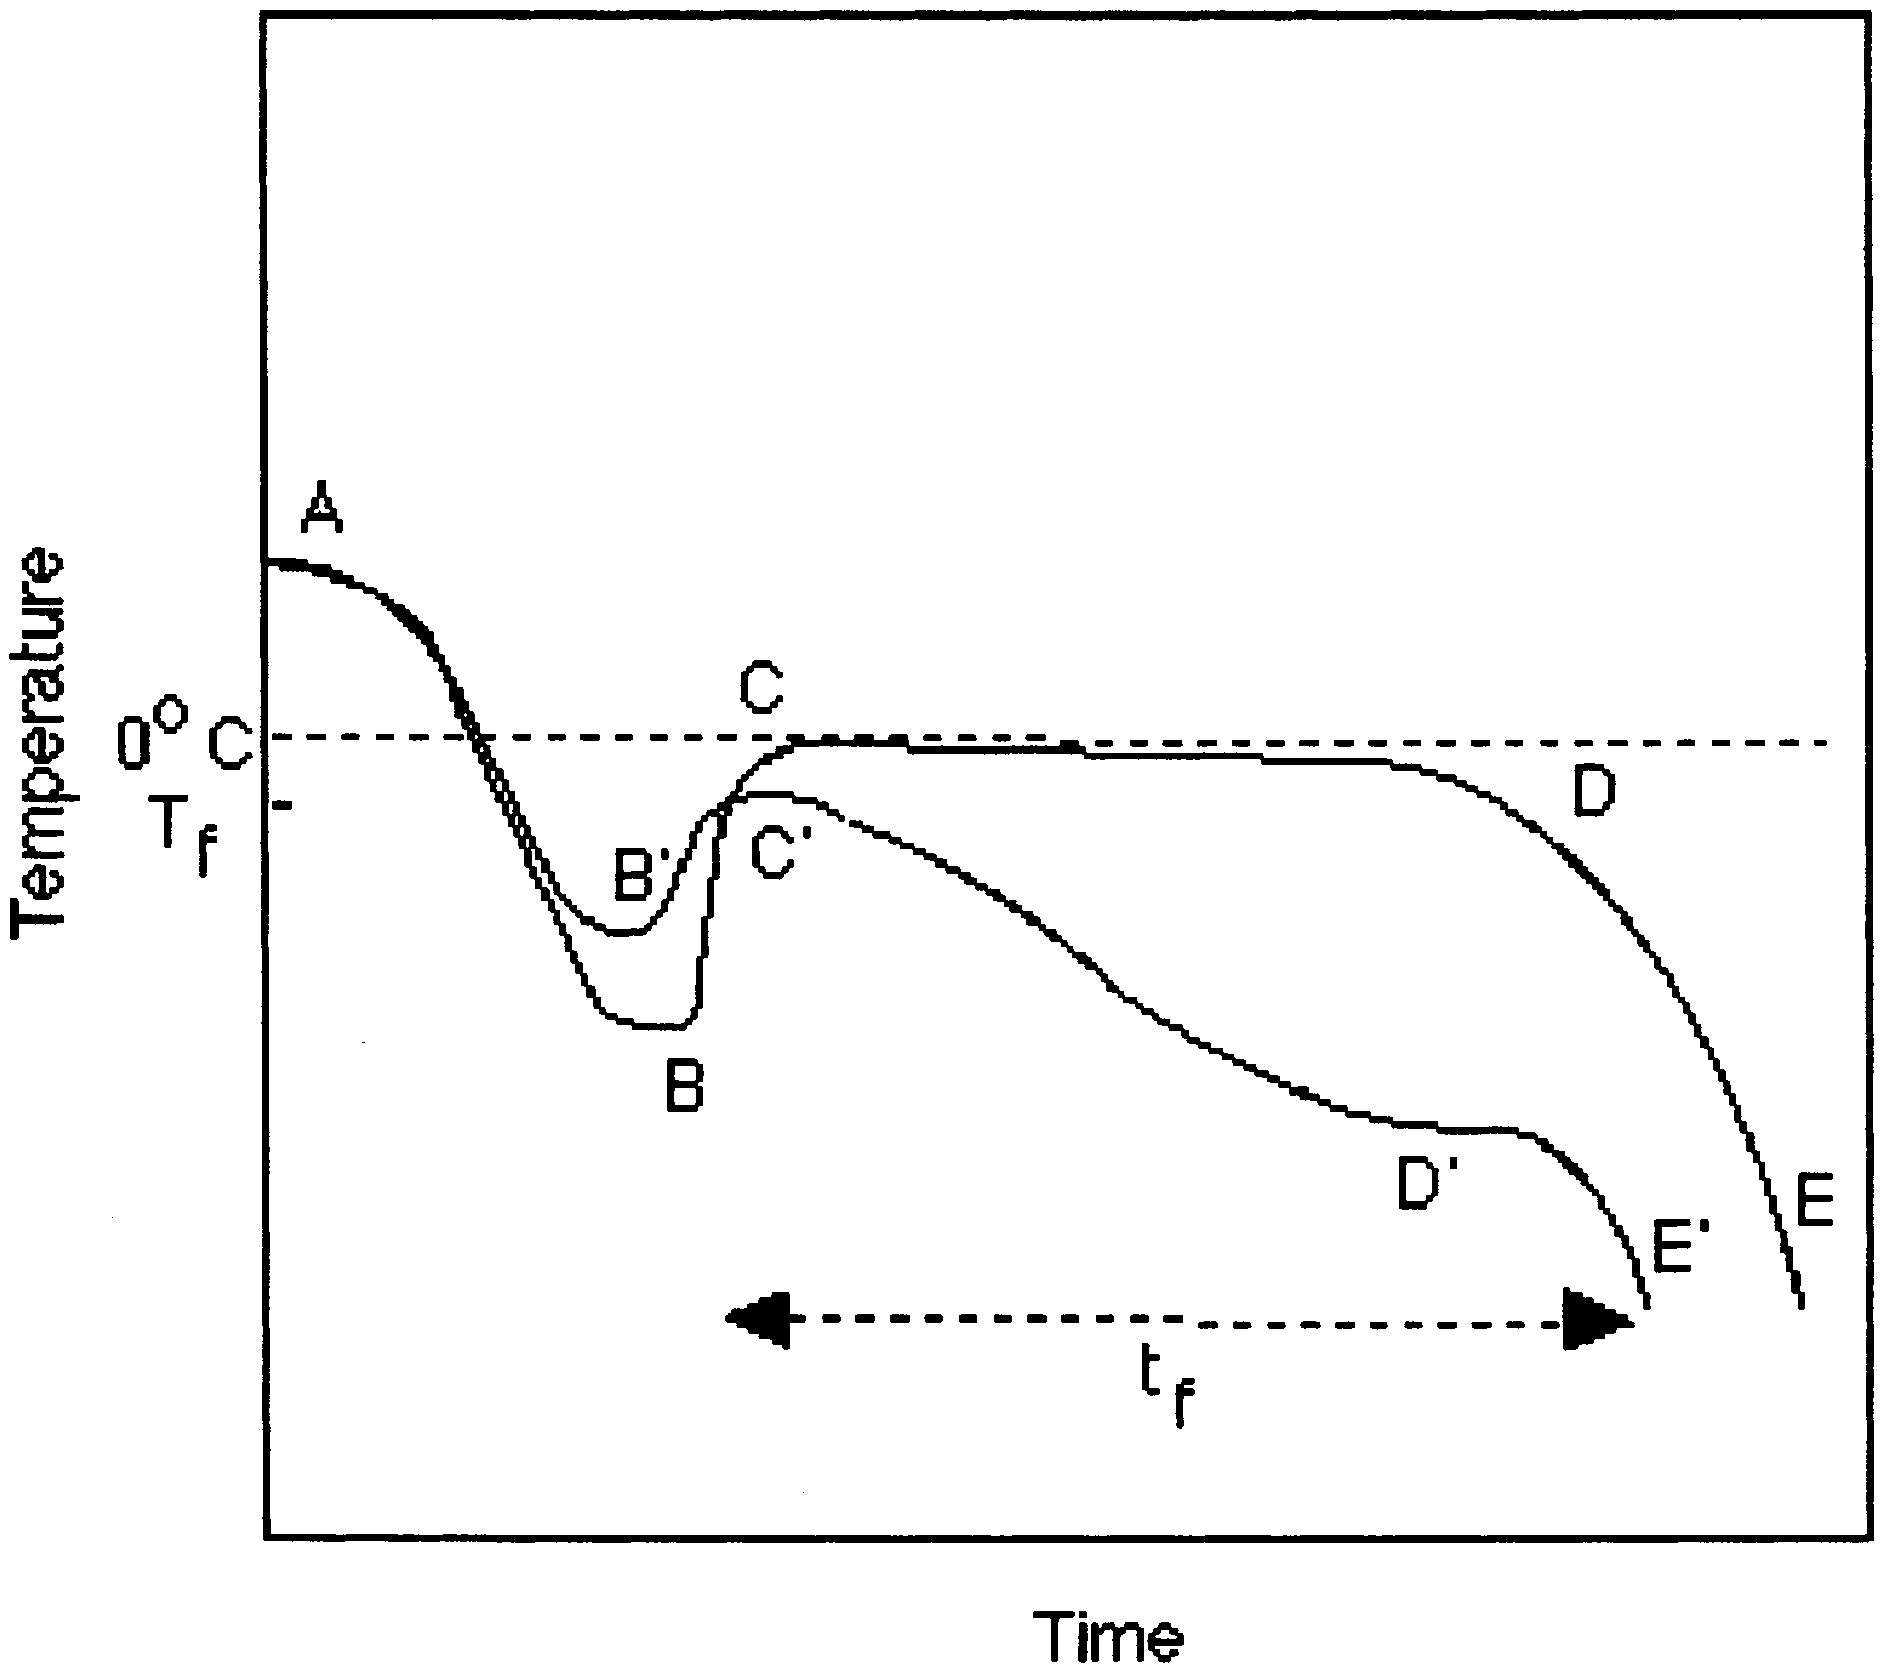
\includegraphics[width=0.6\textwidth]{crystallization_of_water.png}
	\caption{Process of crystallization of water.}
	\label{1.7fig}	
\end{figure} 


\section{Mechanisms of Heat Transfer. Heat convection}

\setlength{\parindent}{0.5cm} In a more generalistic point of view, phase changes occur due to the action of the heat transfer which may appear in the form of convection, conduction or radiation. 

\noindent Convective heat transfer usually occurs in fluids due to the microscopic motion of the particles commonly understood as the bulk fluid motion.

\noindent Depending on the force originating such motion, one can distinguish two types of convection: natural convection and forced convection. Natural convection, the phenomena presented in this thesis, is originated due to differences of temperature gradients. These gradients, in the presence of the gravitational field, allow density to change within the fluid field. At the same time, the fact that density changes, enhances the rise of the colder liquid in contrast with the warmer which tends to sink thus, generating a motion in the fluid. On the other hand, the forced convection is driven by external sources which enforce the motion. In this case, buoyancy is not that relevant as it is for the first kind of convection. 

\noindent In order to model the convection heat transfer in an object, the Newton's cooling law is typically used. As presented in Equation \ref{1.1}:
\begin{equation}
\frac{d Q}{d t}=h A\left(T_{s}(t)-T_{\infty}\right)
\label{1.1}
\end{equation}
where \textit{Q} is the heat source (thermal energy), $T_s$ is the temperature on the surface of the object, $T_{\infty}$ the temperature far away from the object, \textit{h} is the heat transfer coefficient and A, the heat transfer surface area.

\noindent The equation \ref{1.1} states that the rate of heat loss is proportional to the temperature difference between the object itself and the medium by which it is surrounded.

\noindent The process of water freezing in enclosures is common in engineering. When there exist temperature gradients within the liquid phase in the process of solidification, a natural buoyancy driven flow is initiated and such behavior is determined to affect the shape of the liquid/solid interface as well as the progress of solidification.

\noindent Indeed, these temperature differences in the liquid cause density variations so that the natural motion occurs. Boussinesq approximation can be validly used for fluids whose density varies linearly with temperature. However, pure water exhibits a maximum in its density when it ranges between 0ºC and 4ºC. Beyond the latter temperature, and known as density inversion point, density decreases in a nonlinear manner as the temperature passes through the freezing point. In convective heat transfer, surroundings of the temperature where the aforementioned maximum happens to be, behave in a complex manner leading to fully control the process of growth of the solid phase.


\section{Conjugate Heat Transfer. Heat conduction}
\setlength{\parindent}{0.5cm} The other heat transfer mechanism appearing in the thesis is heat conduction which usually happens at molecular level in where the energy is transferred from particles with high energetic levels to lower energetic particles. The equation driving the conductive heat transfer is commonly known as the Fourier's law and it reads as: 
\begin{equation}
	q=-k \nabla T
	\label{1.2}
\end{equation}
where \textit{q} is the heat transfer per unit of area, $\kappa$ is the thermal conductivity of the material and $\nabla T$ is the gradient of temperatures within the studied bodies.

\noindent Alongside, conjugate heat transfer, the phenomena studied in the last part of this thesis, is referred to the heat transfer between solids and fluids. Therefore, a combination of conduction and convection are the main heat transfer mechanisms driving this part of the analysis.


